\documentclass[10pt,twocolumn]{article}
\usepackage[a4paper,margin=0.75in,columnsep=0.25in]{geometry}
\usepackage{times}
\usepackage[T1]{fontenc}
\usepackage{graphicx}
\usepackage{booktabs}
\usepackage{array}
\usepackage{titlesec}
\usepackage{caption}
\captionsetup{font=small,labelfont=bf}
\titleformat{\section}{\normalsize\bfseries\scshape\centering}{\thesection.}{0.5em}{}
\titleformat{\subsection}{\normalsize\itshape}{\thesubsection}{0.5em}{}
\setlength{\parskip}{0pt}
\setlength{\parindent}{1em}

\title{\vspace{-0.4in}\bfseries Counting the Errors That Matter: Silent Wrong Values in Patient-Facing Extraction of Laboratory Reports}
\author{
Keshav Mallawat, Harsh Shah, Guneesh Singh, Atul Pandey, Uday Joshi\\
\small Department of Computer Engineering, K J Somaiya School of Engineering, Somaiya Vidyavihar University, Mumbai, India\\
\small \textit{DRAFT: author list and order to be agreed with the project guide before submission}
}
\date{}

\begin{document}
\maketitle
\vspace{-0.3in}

\begin{abstract}
Patients increasingly receive laboratory results as PDFs and photographs with no explanation, and tools that read and explain them must not mislead. Existing work on extracting laboratory values reports precision, recall and F1, which do not distinguish a missed value from a wrong value displayed with confidence. We define a \emph{silent wrong value}---an incorrect number shown with a confident HIGH, LOW or NORMAL status---and report it as a separate outcome. We describe a deterministic extraction pipeline in which a language model never reads or produces a number, and in which two fail-safes turn doubtful values into ``not compared''. On 1,090 synthetic values with exact ground truth, digital PDFs and lightly degraded scans produced no silent wrong values, while phone-photo quality scans produced 7.2\% (95\% CI 4.3--10.2). An ablation shows that removing the two fail-safes raises this to 16.3\% (11.8--20.9) and introduces silent errors on clear scans. The evidence is synthetic and was produced by the team that built the system; we state what that does and does not support.
\end{abstract}

\noindent\textbf{Keywords:} laboratory report extraction, OCR, patient safety, decision support, health informatics

\section{Introduction}
A person's results are produced in many places and usually reach them as a PDF or a photograph. In a mixed-methods study of 95 adults who received results through an online portal, nearly two thirds received no explanatory information with the result, 46\% searched online for more, and people with abnormal results were more likely to report negative emotions and to call their physician than those with normal results \cite{giardina}. A tool that explains results therefore reaches people who are already anxious, and an error in it is not a minor inconvenience.

Two technologies make such a tool feasible: optical character recognition (OCR) with rule-based or statistical extraction, and large language models that phrase information in plain language. The second carries a specific risk. A preprint evaluating a language-model note-generation workflow found hallucinations in 1.47\% of note sentences, 44\% of them classed as major \cite{llmhalluc}. For a laboratory value, an invented or altered number is the harm itself.

Extraction research reports quality as precision, recall and F1 \cite{ma}. These measures treat a value that is missing and a value that is wrong with confidence as the same kind of error. For a patient-facing tool they are not the same: a missing value is visible, while a wrong value with a confident ``HIGH'' or ``NORMAL'' label looks like a fact.

\textbf{Contributions.} (1) We define the \emph{silent wrong value} and report it separately from recall and accuracy. (2) We describe a deterministic pipeline, implemented in a student project called OneHealth AI, in which a model never produces a number and two fail-safes convert doubtful values into ``not compared''. (3) We measure the pipeline on a reproducible synthetic benchmark and ablate the fail-safes, with document-level confidence intervals.

\section{Related Work}
\textbf{Extraction from laboratory reports.} Ma et al.\ built an OCR and information-extraction pipeline for paper laboratory reports, reporting OCR accuracy of 0.93 and an extraction F1 of 0.86 on 153 reports, with errors from poor scan quality and layout \cite{ma}. Our OCR engine is Tesseract \cite{smith}. We differ in reading digital PDFs from their text layer, in rule-based extraction, and in counting confident errors separately.

\textbf{Negation and context.} ConText assigns negation, temporality and experiencer to clinical conditions \cite{chapman}, and medspaCy packages such methods for spaCy \cite{eyre}. OneHealth AI uses them for conditions, medications and allergies in free text; this paper concerns numeric laboratory values only.

\textbf{Language models in medicine.} Reviews describe benefits and drawbacks of language models in healthcare \cite{thiru}. We take the hallucination risk \cite{llmhalluc} as a design constraint rather than a quantity to estimate.

\section{System}
OneHealth AI has three tiers: a React web application, a Node.js and Express API with a PostgreSQL database, and a Python FastAPI service for document analysis. The analysis service has no database access; the API supplies only what it is permitted to see.

\subsection{Extraction pipeline}
The service reads a PDF's text layer directly, and uses Tesseract for scans and photographs. A table of aliases, including common Indian spellings, matches 14 laboratory parameters (haemoglobin, red and white cell counts, platelets, fasting glucose, HbA1c, creatinine, TSH, total cholesterol, LDL, HDL, triglycerides, ALT, AST). Numbers are parsed, units are normalised (including lakh notation, so ``2,45,000 /cumm'' becomes $245\times10^{3}/\mu$L), and the first number on a line is not accepted as a result if it begins a printed range or follows a ``$<$'' or ``$>$'' sign. Each value keeps its source line.

Reference intervals are fixed constants with a named source (for example WHO haemoglobin thresholds \cite{who}), not model output. A value is classified HIGH, LOW or NORMAL against the interval, selected by the sex printed on the report where the interval differs.

\subsection{Fail-safes}
\textbf{G1, plausibility.} Each parameter has a physiologically plausible window. A value outside it (for example glucose read as 7~mg/dL) is shown as UNKNOWN (``not compared'') and given no status.

\textbf{G2, OCR uncertainty.} In OCR text, a number glued to a preceding non-digit character (for example ``\$7'' where 57 was printed) is shown as UNKNOWN, because the engine may have dropped a digit without any sign in the value itself.

\subsection{Explanation and the role of a model}
The plain-language summary is built deterministically from the extracted values and carries a disclaimer. An optional language model may re-word it; its output is discarded if it contains a number absent from the deterministic draft. A question-answering assistant draws only on the patient's own results and refuses diagnosis, prescription and prognosis before composing an answer. Sharing with a clinician uses a consent lifecycle (pending, approved, rejected, revoked, expired) re-checked on every request, with every access recorded.

\section{Evaluation Method}
\textbf{Data.} Reports are generated from a seeded random generator (seed 20261008), so ground truth is exact. Each lists 8 to 14 of the 14 parameters in one of three layouts (tabular, inline, flagged), with sex-specific values and half the values outside range. Two wording families are used: \emph{known} names listed in the alias table, and \emph{held-out} phrasings written without consulting it. There are 100 documents and 1,090 values: 60 digital PDFs (657 values), 20 clear scans (225), and 20 phone-photo style images (208). Clear scans have small rotation and noise; phone-photo style images are also reduced in size, blurred and heavily JPEG-compressed. Tesseract 5.3.4 is used for OCR.

\textbf{Metrics.} Recall is the share of printed values found. Value accuracy is the share parsed to the right number. A \emph{silent wrong value} is a value returned with a wrong number and a status other than UNKNOWN. A wrong number returned as UNKNOWN is counted as \emph{safely rejected}.

\textbf{Ablation.} The same documents are analysed with G1 removed (the plausibility window widened), G2 removed (OCR flag withheld) and both removed. Each report's text is read once and reused, so only the gates differ. Intervals are 95\% percentile bootstrap over documents (2,000 resamples), because values within one report are not independent.

\section{Results}
Table~\ref{tab:main} gives the main results. Digital PDFs were read without error. Clear scans reached 99.1\% recall and 97.3\% value accuracy with no silent wrong values. At phone-photo quality, recall fell to 75.0\% and value accuracy to 58.7\%, and 15 of 208 values (7.2\%) were silent wrong values. The dominant failure was a digit read as a different digit (for example 142 read as 342), which cannot be detected from the number alone. Value accuracy for held-out wording was 100.0\%, 98.0\% and 62.6\% against 100.0\%, 96.7\% and 55.6\% for known wording, so unseen phrasings did not hurt on this data.

\begin{table}[t]
\centering\small
\caption{Extraction results on synthetic reports.}\label{tab:main}
\begin{tabular}{@{}lrrrr@{}}
\toprule
Input & Values & Recall & Value acc. & Silent wrong\\
\midrule
Digital PDF & 657 & 100.0\% & 100.0\% & 0 (0.0\%)\\
Clear scan & 225 & 99.1\% & 97.3\% & 0 (0.0\%)\\
Phone photo & 208 & 75.0\% & 58.7\% & 15 (7.2\%)\\
\bottomrule
\end{tabular}
\end{table}

Table~\ref{tab:abl} and Fig.~\ref{fig:abl} give the ablation. Value accuracy does not change between rows, because the gates never alter a number; they decide whether it receives a status. At phone-photo quality, removing both gates raised silent wrong values from 15 to 34 (7.2\% to 16.3\%); the intervals (4.3--10.2 and 11.8--20.9) do not overlap. The gates therefore converted 19 of the 34 wrong values (56\%) from confident to visible. On clear scans they converted all 4. G1 contributed more than G2 on this data (29 against 18 silent wrong values when each alone was removed).

\begin{table}[t]
\centering\small
\caption{Silent wrong values with fail-safes removed (count; rate with 95\% CI).}\label{tab:abl}
\begin{tabular}{@{}lcc@{}}
\toprule
Gates & Clear scan & Phone photo\\
\midrule
Both on (shipped) & 0 (0.0) & 15 (7.2; 4.3--10.2)\\
G1 removed & 3 (1.3; 0.0--2.8) & 29 (13.9; 9.9--18.0)\\
G2 removed & 1 (0.4; 0.0--1.4) & 18 (8.7; 5.6--11.7)\\
Both removed & 4 (1.8; 0.0--4.0) & 34 (16.3; 11.8--20.9)\\
\bottomrule
\end{tabular}
\end{table}

\begin{figure}[t]
\centering
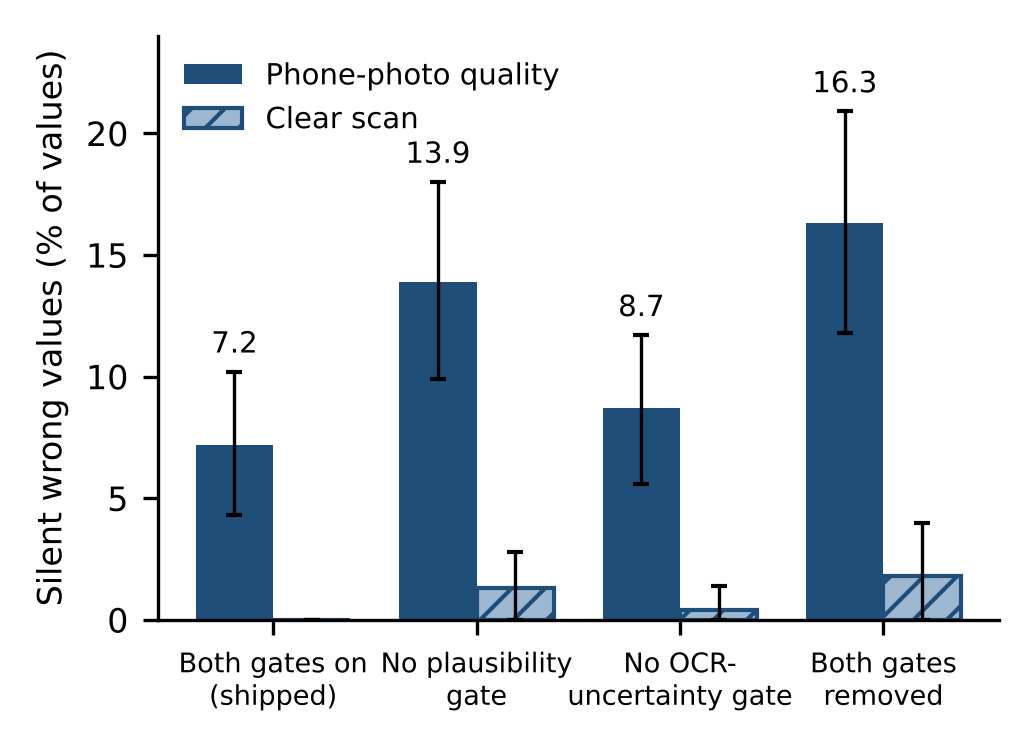
\includegraphics[width=\columnwidth]{fig-ablation.png}
\caption{Silent wrong values by fail-safe configuration. Error bars are 95\% document-level bootstrap intervals. Digital PDFs had none in any configuration.}\label{fig:abl}
\end{figure}

\section{Limitations}
\textbf{The data are synthetic and team-written.} The benchmark shows the extractor is reliable on the layouts and wording families tested; it does not show accuracy on any laboratory's real format. Degradation is simulated, not photographed.

\textbf{The system was tuned on this benchmark.} The first run exposed six extractor faults, including one that reported an LDL value as total cholesterol; they were fixed and the benchmark re-run, raising value accuracy on clear scans from 87.6\% to 97.3\%. The reported numbers are therefore optimistic for unseen data. Held-out wording reduces but does not remove this concern, because layouts and degradation are shared.

\textbf{Other limits.} The 20-document groups give wide intervals. Status accuracy uses the project's own reference intervals, so it tests the logic, not the clinical correctness of the intervals. We evaluate 14 parameters in English with no real patients and no user study. Timing was measured on a cloud CPU without the network hop. The system is a decision-support aid and not a diagnostic tool.

\section{Conclusion}
Reporting silent wrong values separately makes visible a failure that F1 hides. In a deterministic pipeline, two simple fail-safes roughly halved confident errors on poor scans and removed them on clear scans, at no cost in accuracy, but phone-quality photographs remain unsafe to read unattended. Future work includes evaluating on real, consented and ethically approved reports; cross-checking each value against the status printed on the report; comparison with a learned extractor such as the conditional-random-field method of Ma et al.\ \cite{ma}; and mapping extracted values to FHIR Observation resources.

\begin{thebibliography}{9}\small
\bibitem{giardina} T. D. Giardina, J. Baldwin, D. T. Nystrom, D. F. Sittig and H. Singh, ``Patient perceptions of receiving test results via online portals: a mixed-methods study,'' \emph{J. Am. Med. Inform. Assoc.}, vol. 25, no. 4, pp. 440--446, 2018.
\bibitem{ma} M.-W. Ma, X.-S. Gao, Z.-Y. Zhang et al., ``Extracting laboratory test information from paper-based reports,'' \emph{BMC Med. Inform. Decis. Mak.}, vol. 23, art. 251, 2023.
\bibitem{smith} R. Smith, ``An overview of the Tesseract OCR engine,'' in \emph{Proc. 9th Int. Conf. Document Analysis and Recognition (ICDAR)}, 2007, pp. 629--633.
\bibitem{chapman} W. W. Chapman, D. Chu and J. N. Dowling, ``ConText: an algorithm for identifying contextual features from clinical text,'' in \emph{Proc. BioNLP Workshop}, Prague, 2007, pp. 81--88.
\bibitem{eyre} H. Eyre et al., ``Launching into clinical space with medspaCy: a new clinical text processing toolkit in Python,'' in \emph{AMIA Annu. Symp. Proc.}, 2022.
\bibitem{thiru} A. J. Thirunavukarasu et al., ``Large language models in medicine,'' \emph{Nat. Med.}, vol. 29, pp. 1930--1940, 2023.
\bibitem{llmhalluc} ``A framework to assess clinical safety and hallucination rates of LLMs for medical text summarisation,'' medRxiv preprint, 2024, doi:10.1101/2024.09.12.24313556. [AUTHORS TO BE CONFIRMED BEFORE SUBMISSION]
\bibitem{who} World Health Organization, ``Haemoglobin concentrations for the diagnosis of anaemia and assessment of severity,'' WHO/NMH/NHD/MNM/11.1, 2011.
\end{thebibliography}
\end{document}
